% Options for packages loaded elsewhere
\PassOptionsToPackage{unicode}{hyperref}
\PassOptionsToPackage{hyphens}{url}
\documentclass[
  ignorenonframetext,
]{beamer}
\newif\ifbibliography
\usepackage{pgfpages}
\setbeamertemplate{caption}[numbered]
\setbeamertemplate{caption label separator}{: }
\setbeamercolor{caption name}{fg=normal text.fg}
\beamertemplatenavigationsymbolsempty
% remove section numbering
\setbeamertemplate{part page}{
  \centering
  \begin{beamercolorbox}[sep=16pt,center]{part title}
    \usebeamerfont{part title}\insertpart\par
  \end{beamercolorbox}
}
\setbeamertemplate{section page}{
  \centering
  \begin{beamercolorbox}[sep=12pt,center]{section title}
    \usebeamerfont{section title}\insertsection\par
  \end{beamercolorbox}
}
\setbeamertemplate{subsection page}{
  \centering
  \begin{beamercolorbox}[sep=8pt,center]{subsection title}
    \usebeamerfont{subsection title}\insertsubsection\par
  \end{beamercolorbox}
}
% Prevent slide breaks in the middle of a paragraph
\widowpenalties 1 10000
\raggedbottom
\AtBeginPart{
  \frame{\partpage}
}
\AtBeginSection{
  \ifbibliography
  \else
    \frame{\sectionpage}
  \fi
}
\AtBeginSubsection{
  \frame{\subsectionpage}
}
\usepackage{iftex}
\ifPDFTeX
  \usepackage[T1]{fontenc}
  \usepackage[utf8]{inputenc}
  \usepackage{textcomp} % provide euro and other symbols
\else % if luatex or xetex
  \usepackage{unicode-math} % this also loads fontspec
  \defaultfontfeatures{Scale=MatchLowercase}
  \defaultfontfeatures[\rmfamily]{Ligatures=TeX,Scale=1}
\fi
\usepackage{lmodern}
\ifPDFTeX\else
  % xetex/luatex font selection
\fi
% Use upquote if available, for straight quotes in verbatim environments
\IfFileExists{upquote.sty}{\usepackage{upquote}}{}
\IfFileExists{microtype.sty}{% use microtype if available
  \usepackage[]{microtype}
  \UseMicrotypeSet[protrusion]{basicmath} % disable protrusion for tt fonts
}{}
\makeatletter
\@ifundefined{KOMAClassName}{% if non-KOMA class
  \IfFileExists{parskip.sty}{%
    \usepackage{parskip}
  }{% else
    \setlength{\parindent}{0pt}
    \setlength{\parskip}{6pt plus 2pt minus 1pt}}
}{% if KOMA class
  \KOMAoptions{parskip=half}}
\makeatother
\usepackage{color}
\usepackage{fancyvrb}
\newcommand{\VerbBar}{|}
\newcommand{\VERB}{\Verb[commandchars=\\\{\}]}
\DefineVerbatimEnvironment{Highlighting}{Verbatim}{commandchars=\\\{\}}
% Add ',fontsize=\small' for more characters per line
\newenvironment{Shaded}{}{}
\newcommand{\AlertTok}[1]{\textcolor[rgb]{1.00,0.00,0.00}{\textbf{#1}}}
\newcommand{\AnnotationTok}[1]{\textcolor[rgb]{0.38,0.63,0.69}{\textbf{\textit{#1}}}}
\newcommand{\AttributeTok}[1]{\textcolor[rgb]{0.49,0.56,0.16}{#1}}
\newcommand{\BaseNTok}[1]{\textcolor[rgb]{0.25,0.63,0.44}{#1}}
\newcommand{\BuiltInTok}[1]{\textcolor[rgb]{0.00,0.50,0.00}{#1}}
\newcommand{\CharTok}[1]{\textcolor[rgb]{0.25,0.44,0.63}{#1}}
\newcommand{\CommentTok}[1]{\textcolor[rgb]{0.38,0.63,0.69}{\textit{#1}}}
\newcommand{\CommentVarTok}[1]{\textcolor[rgb]{0.38,0.63,0.69}{\textbf{\textit{#1}}}}
\newcommand{\ConstantTok}[1]{\textcolor[rgb]{0.53,0.00,0.00}{#1}}
\newcommand{\ControlFlowTok}[1]{\textcolor[rgb]{0.00,0.44,0.13}{\textbf{#1}}}
\newcommand{\DataTypeTok}[1]{\textcolor[rgb]{0.56,0.13,0.00}{#1}}
\newcommand{\DecValTok}[1]{\textcolor[rgb]{0.25,0.63,0.44}{#1}}
\newcommand{\DocumentationTok}[1]{\textcolor[rgb]{0.73,0.13,0.13}{\textit{#1}}}
\newcommand{\ErrorTok}[1]{\textcolor[rgb]{1.00,0.00,0.00}{\textbf{#1}}}
\newcommand{\ExtensionTok}[1]{#1}
\newcommand{\FloatTok}[1]{\textcolor[rgb]{0.25,0.63,0.44}{#1}}
\newcommand{\FunctionTok}[1]{\textcolor[rgb]{0.02,0.16,0.49}{#1}}
\newcommand{\ImportTok}[1]{\textcolor[rgb]{0.00,0.50,0.00}{\textbf{#1}}}
\newcommand{\InformationTok}[1]{\textcolor[rgb]{0.38,0.63,0.69}{\textbf{\textit{#1}}}}
\newcommand{\KeywordTok}[1]{\textcolor[rgb]{0.00,0.44,0.13}{\textbf{#1}}}
\newcommand{\NormalTok}[1]{#1}
\newcommand{\OperatorTok}[1]{\textcolor[rgb]{0.40,0.40,0.40}{#1}}
\newcommand{\OtherTok}[1]{\textcolor[rgb]{0.00,0.44,0.13}{#1}}
\newcommand{\PreprocessorTok}[1]{\textcolor[rgb]{0.74,0.48,0.00}{#1}}
\newcommand{\RegionMarkerTok}[1]{#1}
\newcommand{\SpecialCharTok}[1]{\textcolor[rgb]{0.25,0.44,0.63}{#1}}
\newcommand{\SpecialStringTok}[1]{\textcolor[rgb]{0.73,0.40,0.53}{#1}}
\newcommand{\StringTok}[1]{\textcolor[rgb]{0.25,0.44,0.63}{#1}}
\newcommand{\VariableTok}[1]{\textcolor[rgb]{0.10,0.09,0.49}{#1}}
\newcommand{\VerbatimStringTok}[1]{\textcolor[rgb]{0.25,0.44,0.63}{#1}}
\newcommand{\WarningTok}[1]{\textcolor[rgb]{0.38,0.63,0.69}{\textbf{\textit{#1}}}}
\usepackage{graphicx}
\makeatletter
\newsavebox\pandoc@box
\newcommand*\pandocbounded[1]{% scales image to fit in text height/width
  \sbox\pandoc@box{#1}%
  \Gscale@div\@tempa{\textheight}{\dimexpr\ht\pandoc@box+\dp\pandoc@box\relax}%
  \Gscale@div\@tempb{\linewidth}{\wd\pandoc@box}%
  \ifdim\@tempb\p@<\@tempa\p@\let\@tempa\@tempb\fi% select the smaller of both
  \ifdim\@tempa\p@<\p@\scalebox{\@tempa}{\usebox\pandoc@box}%
  \else\usebox{\pandoc@box}%
  \fi%
}
% Set default figure placement to htbp
\def\fps@figure{htbp}
\makeatother
\setlength{\emergencystretch}{3em} % prevent overfull lines
\providecommand{\tightlist}{%
  \setlength{\itemsep}{0pt}\setlength{\parskip}{0pt}}
% Slide layout defaults for warning-clean scientific decks.
\usepackage{etoolbox}
\IfFileExists{xurl.sty}{\usepackage{xurl}}{}
\IfFileExists{seqsplit.sty}{\usepackage{seqsplit}}{\newcommand{\seqsplit}[1]{#1}}
\protected\def\breakseq#1{\seqsplit{#1}}
\protected\def\breaktt#1{\begingroup\ttfamily\seqsplit{#1}\endgroup}
\setlength{\emergencystretch}{6em}
\tolerance=5000
\hbadness=10000
\hfuzz=1pt
\setlength{\tabcolsep}{2pt}
\AtBeginEnvironment{longtable}{\tiny\renewcommand{\arraystretch}{0.86}\setlength{\tabcolsep}{1pt}}
\AtBeginEnvironment{tabular}{\tiny\renewcommand{\arraystretch}{0.86}\setlength{\tabcolsep}{1pt}}

% Natbib and cross-reference fallbacks — slides don't load natbib
% or cleveref, but combined-PDF manuscript prose may emit these
% commands. The fallback renders citations as a bracketed key list
% and cross-references as detokenized labels so slides don't fail on
% undefined control sequences or raw underscores. \providecommand is
% a no-op if packages load later.
\providecommand{\citep}[1]{[#1]}
\providecommand{\citet}[1]{#1}
\providecommand{\citealp}[1]{#1}
\providecommand{\citeauthor}[1]{#1}
\providecommand{\citeyear}[1]{#1}
\providecommand{\cref}[1]{\texttt{\detokenize{#1}}}
\providecommand{\Cref}[1]{\texttt{\detokenize{#1}}}
\usepackage{bookmark}
\IfFileExists{xurl.sty}{\usepackage{xurl}}{} % add URL line breaks if available
\urlstyle{same}
% fallback for those not using the hyperref driver hyperxmp:
\makeatletter
\@ifundefined{xmpquote}{\newcommand{\xmpquote}[1]{#1}}{}
\makeatother
\hypersetup{
  hidelinks,
  pdfcreator={LaTeX via pandoc}}

\author{\texorpdfstring{}{}}
\date{}

\begin{document}

\section{Methodology}\label{sec:methodology}

\begin{frame}[fragile,allowframebreaks]{Methodology}
Two distinct workflows run on top of
\breaktt{infrastructure/search/literature} and
\breaktt{infrastructure/reference/citation}:

\begin{itemize}
\tightlist
\item
  \textbf{Standard pipeline} (\breaktt{scripts/run\_search\_pipeline.py}
  → \breaktt{src/pipeline.py::run\_literature\_pipeline}) --- single
  \texttt{SearchQuery}. Four pure-orchestration stages with no LLM
  dependency: (1) search via \breaktt{LiteratureClient}, (2) enrichment
  via \texttt{AbstractFetcher} and (optional) \texttt{FulltextFetcher},
  (3) collision-free citation-key generation in
  \breaktt{\_build\_citation\_keys}, (4) writing
  \breaktt{output/corpus.json} + \breaktt{manuscript/references.bib} +
  \breaktt{output/enrichment\_log.json}. The orchestrator script then
  optionally calls \breaktt{src/synthesis.py} for per-paper and corpus
  LLM synthesis and \texttt{src/report.py} for the final reading report.
\item
  \textbf{Deep search} (\breaktt{scripts/run\_deep\_search.py} →
  \breaktt{src/deep\_search.py::run\_deep\_search}) --- multi-keyword
  fan-out: each keyword runs its own \texttt{SearchQuery} capped at
  \breaktt{max\_results\_per\_keyword} (100 by default), every paper is
  fully enriched (abstract + PDF fulltext when available), and an
  LLM-driven multi-section deep summary (CONTRIBUTION / METHOD /
  EVIDENCE / LIMITATIONS / CONNECTIONS / SIGNIFICANCE / TAGS) is written
  for each paper as a standalone markdown reading note. Output lands
  under
  \texttt{output/deep\_search/\textless{}keyword\_slug\textgreater{}/}
  plus aggregate \texttt{aggregate.json}, \breaktt{aggregate\_report.md},
  and a unified, deduplicated \breaktt{manuscript/references\_deep.bib}
  with collision-free citation keys.
\end{itemize}

The standard pipeline is described first in this section; the
deep-search workflow is documented in \breakseq{[@sec:deep\_search]}.
Diagnostic figures for the latest pipeline run appear at the end of this
section.
\end{frame}

\begin{frame}[fragile,allowframebreaks]{Search}
\protect\phantomsection\label{search}
The search stage is intentionally faithful to the standard
literature-search pattern documented in foundational optimisation
textbooks \breakseq{[@boyd2004convex; @nocedal2006numerical]} --- a
deterministic query, capped result count, and explicit failure isolation
between sources --- so reviewers familiar with those references can
reason about the workflow without learning new abstractions.

A \texttt{SearchQuery} is constructed from \texttt{config.search}:

\begin{Shaded}
\begin{Highlighting}[]
\NormalTok{SearchQuery(}
\NormalTok{    text}\OperatorTok{=}\NormalTok{config.search.query,}
\NormalTok{    max\_results}\OperatorTok{=}\NormalTok{config.search.max\_results,}
\NormalTok{    year\_min}\OperatorTok{=}\NormalTok{config.search.year\_min,}
\NormalTok{    year\_max}\OperatorTok{=}\NormalTok{config.search.year\_max,}
\NormalTok{)}
\end{Highlighting}
\end{Shaded}

A \breaktt{LiteratureClient} is constructed with the configured backends.
Each backend produces a normalised \texttt{Paper} record; the aggregator
deduplicates by DOI → arXiv id → normalised (title, year), keeping the
highest-scored copy and filling missing fields from the loser.

Per-backend errors are recorded into \breaktt{SearchResult.errors} rather
than raised. A network outage in one backend never breaks the workflow;
partial coverage is reported by the final stage.
\end{frame}

\begin{frame}[fragile,allowframebreaks]{Cache}
\protect\phantomsection\label{cache}
\texttt{SearchCache} writes one JSON file per query, named by a
16-character SHA-256 prefix of the canonical query identity. Identical
queries (modulo whitespace and case) share a cache entry. Cache files
are pretty-printed JSON, version-control-friendly, and contain a
\texttt{\_cached\_at} timestamp for optional TTL enforcement.
\end{frame}

\begin{frame}[fragile,allowframebreaks]{Enrichment}
\protect\phantomsection\label{enrichment}
Two fetchers populate fields the search backends did not supply:

\begin{itemize}
\tightlist
\item
  \texttt{AbstractFetcher} --- currently fetches arXiv abstracts via the
  export API, writes them to
  \texttt{\textless{}safe\_id\textgreater{}.txt} under the configured
  cache directory, and re-uses them on subsequent runs.
\item
  \texttt{FulltextFetcher} --- downloads PDFs (arXiv URL,
  \texttt{paper.pdf\_url}, or a caller-supplied override), writes the
  bytes verbatim to \texttt{\textless{}safe\_id\textgreater{}.pdf}, and
  extracts text via \texttt{pypdf} to
  \texttt{\textless{}safe\_id\textgreater{}.txt}. Without \texttt{pypdf}
  the PDF is still cached, and the fetcher returns
  \texttt{status="error"} with an informative message; the rest of the
  pipeline continues.
\end{itemize}

Both fetchers stamp \texttt{paper.abstract} / \texttt{paper.fulltext} in
place, so downstream stages see enriched records without re-loading.
\end{frame}

\begin{frame}[fragile,allowframebreaks]{Export}
\protect\phantomsection\label{export}
For every paper, \breaktt{paper\_to\_bibentry()} produces a
\texttt{BibEntry} whose:

\begin{itemize}
\tightlist
\item
  citation key follows the exemplar's
  \texttt{\textless{}author\textgreater{}\textless{}year\textgreater{}\textless{}title-word\textgreater{}}
  convention with stop-word filtering and unicode folding;
\item
  entry type is routed by \texttt{venue\_type} (journal →
  \texttt{@article}, conference → \texttt{@inproceedings}, book →
  \texttt{@book}, preprint → \texttt{@article}, etc.);
\item
  fields are emitted in the order observed in \texttt{references.bib}:
  title, author, journal/booktitle, year, volume, number, pages,
  publisher, edition, isbn, doi, url, abstract, keywords.
\end{itemize}

A \texttt{BibDatabase} collects these entries and
\texttt{write\_bibfile} renders them in the project's house format:
2-space indent, trailing-comma rule, \texttt{pages=\{N-\/-M\}}, verbatim
DOIs/years, bare unicode.
\end{frame}

\begin{frame}[fragile,allowframebreaks]{Synthesis}
\protect\phantomsection\label{synthesis}
Two LLM passes produce the reading report (see
\breaktt{src/synthesis.py}):

\begin{itemize}
\tightlist
\item
  \textbf{Per-paper synthesis} ---
  \breaktt{build\_paper\_block(paper,\ citation\_key,\ max\_fulltext=4000)}
  renders the paper as a markdown block; \breaktt{synthesise\_per\_paper}
  formats \breaktt{PROMPT\_PER\_PAPER} and calls the injected
  \texttt{llm} callable. The prompt requests five sections:
  CONTRIBUTION, METHOD, EVIDENCE, LIMITATION, TAGS, plus a citation-key
  reference.
\item
  \textbf{Corpus synthesis} --- \breaktt{build\_corpus\_block}
  concatenates every paper into a single citation-keyed block;
  \breaktt{synthesise\_corpus} formats \texttt{PROMPT\_CORPUS}, which
  asks for 3--7 thematic clusters, methodological agreements /
  disagreements (≥ 2 papers each), and three open questions that the
  corpus does not answer.
\end{itemize}

Both functions return a
\breaktt{SynthesisResult(kind,\ prompt,\ text,\ paper\_id)} record so the
prompt is recoverable for reproducibility. The synthesis layer takes a
callable \texttt{llm:\ (str)\ -\textgreater{}\ str} so tests pass a
deterministic local function (no Ollama dependency) and runtime callers
pass a thin adapter around \breaktt{infrastructure.llm.LLMClient}.
Determinism in production runs is enforced by
\breaktt{OllamaClientConfig(seed=42,\ temperature=0.0)}.

The deep-search workflow uses a richer prompt
(\breaktt{src/deep\_search.py::DEEP\_PROMPT}) with seven sections
(CONTRIBUTION / METHOD / EVIDENCE / LIMITATIONS / CONNECTIONS /
SIGNIFICANCE / TAGS) and a much larger \texttt{max\_fulltext} budget
(400 k chars by default).
\end{frame}

\begin{frame}[fragile,allowframebreaks]{Report}
\protect\phantomsection\label{report}
\breaktt{src/report.py::write\_reading\_report} assembles a markdown file
with:

\begin{itemize}
\tightlist
\item
  Topic, result count, year filter, and any backend errors at the top.
\item
  A per-source count table.
\item
  One-line summaries for every paper.
\item
  The corpus synthesis (if present).
\item
  All per-paper notes (if present).
\end{itemize}

Citation keys appear in \texttt{{[}brackets{]}} so a downstream tool ---
for example a Pandoc filter or a manual search --- can resolve them
against the auto-generated \texttt{references.bib}.
\end{frame}

\begin{frame}[fragile,allowframebreaks]{Diagnostic figures}
\protect\phantomsection\label{diagnostic-figures}
\breaktt{scripts/y\_generate\_search\_figures.py} (a thin orchestrator
over \texttt{src/figures.py}) writes three diagnostic plots into
\texttt{output/figures/} from \breaktt{output/search/results.json}. Each
figure uses Matplotlib's \texttt{Agg} backend so the pipeline runs
headlessly in CI; the colour palette is colourblind-safe (Wong,
\emph{Nature Methods} 2011).

\breakseq{[@fig:papers\_per\_source]} reports the per-backend contribution
counts before deduplication, surfacing which sources actually returned
coverage for the configured query. The bar values are read directly from
\breaktt{SearchResult.per\_source\_counts} (set by
\breaktt{LiteratureClient} \emph{before} the DOI / arXiv-id / title merge
step), so a backend that returned five papers all duplicating arXiv hits
still scores five here.

\begin{figure}
\centering
\pandocbounded{\includegraphics[keepaspectratio,alt={Per-source paper counts read from SearchResult.per\_source\_counts (pre-deduplication contribution per backend). The numeric label above each bar reports the raw count; the y-axis spans {[}0, max + headroom{]}. Bar order follows the order recorded in config.search.sources. Empty runs render (no results) centred. Generated by src/figures.py::plot\_papers\_per\_source.}]{../figures/papers_per_source.png}}
\caption{Per-source paper counts read from
\protect\breaktt{SearchResult.per\_source\_counts} (pre-deduplication
contribution per backend). The numeric label above each bar reports the
raw count; the y-axis spans \protect\texttt{{[}0,\ max\ +\ headroom{]}}.
Bar order follows the order recorded in
\protect\breaktt{config.search.sources}. Empty runs render
\protect\texttt{(no\ results)} centred. Generated by
\protect\breaktt{src/figures.py::plot\_papers\_per\_source}.}\label{fig:papers_per_source}
\end{figure}

\breakseq{[@fig:year\_histogram]} shows the publication-year distribution
\emph{after} the merge step (one bar per unique paper, not per backend
hit) --- useful for spotting backend coverage gaps in older / newer
literature. Papers with no \texttt{year} field are dropped silently from
the histogram (they remain in the corpus).

\begin{figure}
\centering
\pandocbounded{\includegraphics[keepaspectratio,alt={Publication-year histogram of the deduplicated paper roster. One bin per year (no smoothing); the x-axis spans the observed {[}min(year), max(year){]} from result.papers. Papers with year is None are dropped; the y-axis is per-year paper count. Generated by src/figures.py::plot\_year\_histogram.}]{../figures/year_histogram.png}}
\caption{Publication-year histogram of the deduplicated paper roster.
One bin per year (no smoothing); the x-axis spans the observed
\protect\texttt{{[}min(year),\ max(year){]}} from
\protect\texttt{result.papers}. Papers with
\protect\texttt{year\ is\ None} are dropped; the y-axis is per-year
paper count. Generated by
\protect\breaktt{src/figures.py::plot\_year\_histogram}.}\label{fig:year_histogram}
\end{figure}

\breakseq{[@fig:score\_distribution]} shows the per-paper relevance scores
returned by the backends, ranked descending. Papers from backends
without an explicit ranking signal (e.g.~\texttt{LocalBackend}, the
offline default) carry \breaktt{Paper.score\ =\ 0.0}; their bars
therefore have zero length but still appear as ticks on the y-axis so
the reader can see how many unranked papers exist.

\begin{figure}
\centering
\pandocbounded{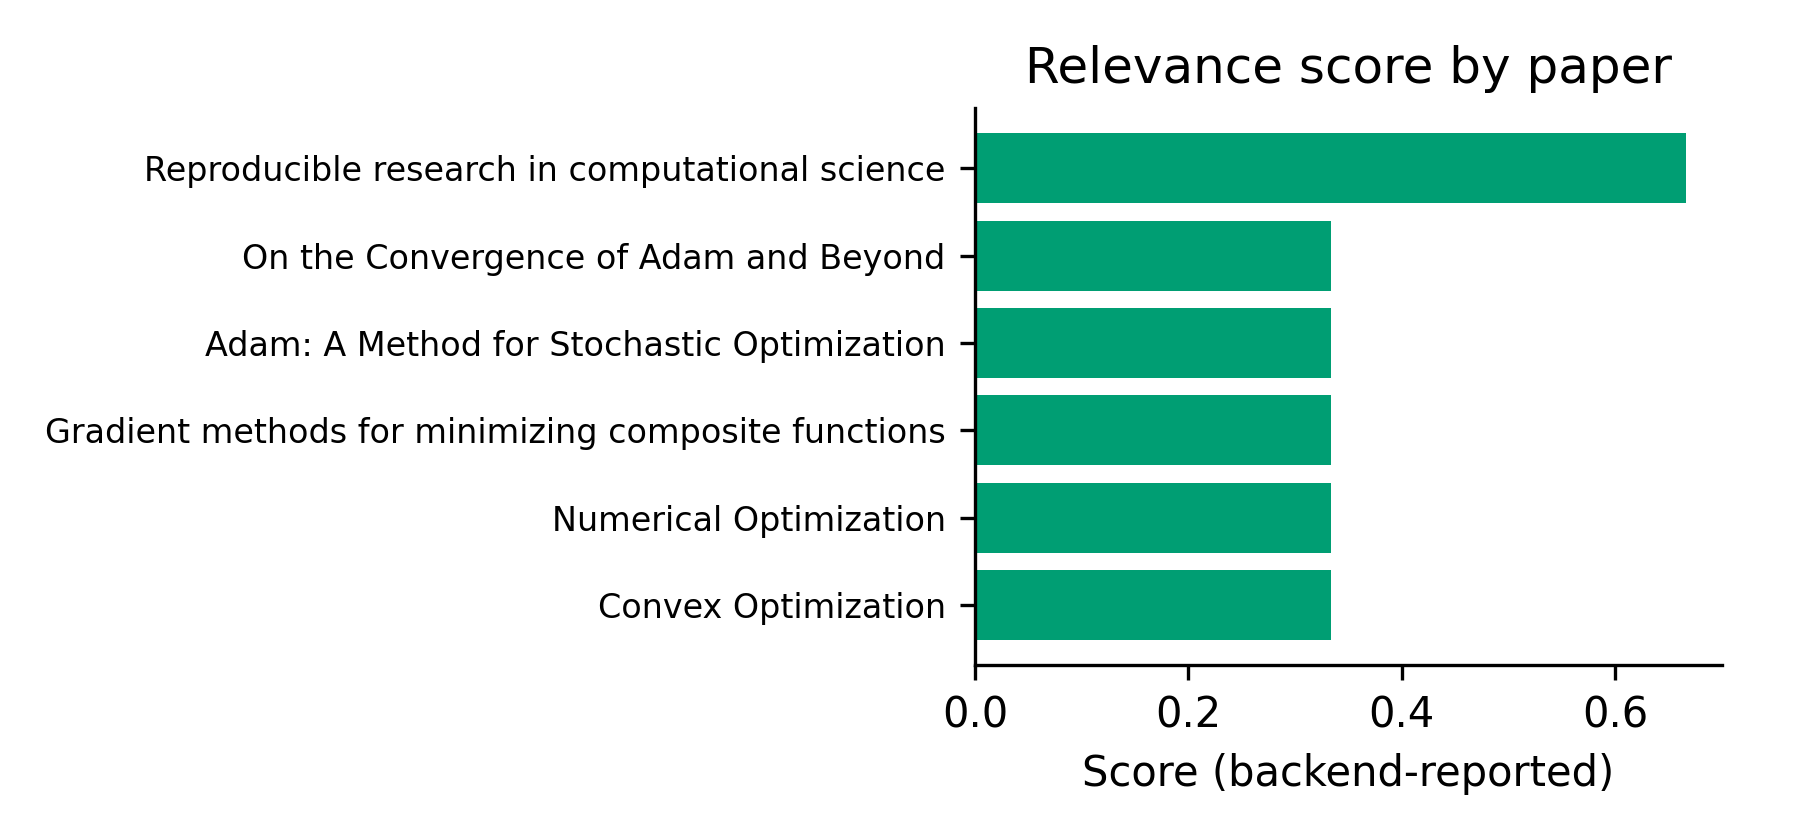
\includegraphics[keepaspectratio,alt={Per-paper backend-reported relevance scores ranked descending (highest at top). Each horizontal bar is one Paper.score; the y-tick label is the paper title truncated to 60 characters with an ellipsis. Backends without scoring (notably LocalBackend) report Paper.score = 0.0 so those bars have zero length. Generated by src/figures.py::plot\_score\_distribution.}]{../figures/score_distribution.png}}
\caption{Per-paper backend-reported relevance scores ranked descending
(highest at top). Each horizontal bar is one
\protect\texttt{Paper.score}; the y-tick label is the paper title
truncated to 60 characters with an ellipsis. Backends without scoring
(notably \protect\texttt{LocalBackend}) report
\protect\breaktt{Paper.score\ =\ 0.0} so those bars have zero length.
Generated by
\protect\breaktt{src/figures.py::plot\_score\_distribution}.}\label{fig:score_distribution}
\end{figure}
\end{frame}

\end{document}
